\documentclass{scrartcl}
\usepackage{amssymb}
\usepackage{amsmath}
\usepackage{tikz}
\usetikzlibrary{calc,intersections,through,backgrounds,patterns}
\usetikzlibrary{decorations.text, decorations.markings, fit}
\usepackage{textcomp}

\begin{document}

%\begin{figure}
%	\centering
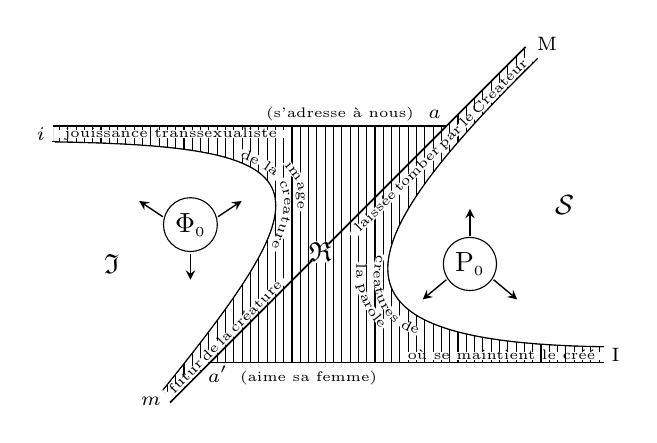
\begin{tikzpicture}

%note: primes (e.g. x') are by convention lower than x
\coordinate (a') at (0,0) {};
\coordinate (a)  at (3,3) {};
\coordinate (M)  at (4,4) {};			%top right
\coordinate (M') at (4.15,3.85) {};
\coordinate (q)  at (-2,3) {};			%top left
\coordinate (q') at (-2,2.8) {};
\coordinate (I') at (5,0) {};			%bottom right
\coordinate (I)  at (5,0.2) {};
\coordinate (m)  at (-0.6,-0.35) {};	%bottom left
\coordinate (m') at (-0.5,-0.5) {};
\coordinate (i)  at (1.5,3) {};

%outside labels
\node at (-2.15,2.9) {{\scriptsize $i$}};
\node at (-0.75,-0.5) {{\scriptsize $m$}};
\node at (4.28,4.05) {{\scriptsize M}};
\node at (5.15,0.1) {{\scriptsize I}};
\node at (0.1,-0.15) {{\scriptsize $a^\prime$}};
\node at (1.25,-0.2) {{\tiny (aime sa femme)}};
\node at (2.85,3.15) {{\scriptsize $a$}};
\node at (1.65,3.15) {{\tiny (s'adresse \`{a} nous)}};
%\node at (1,0) {a};

%outer lines
\draw [semithick]	(a')--(I');
\draw [semithick]	(a')--(M);
\draw [semithick]	(a')--(m');
\draw [semithick]	(q)--(a);
%\draw [semithick] 	(m)--(q');		%temporary line
%\draw [semithick] 	(I)--(M');		%temporary line
%
%curved lines
\draw (m) .. controls (1.5,2.25) and (1.5,2.75) .. (q');
\draw (I) .. controls (1.5,0.25) and (1.5,1.25) .. (M');

%TO DO: make hatch spacing denser
%hatching
\draw[pattern=vertical lines, pattern color=black] (q)--(q')--(m)--(m')--(a);
\draw[pattern=vertical lines, pattern color=black] (a')--(M)--(M')--(I)--(I');

%more outer lines (white)
\draw [semithick, white]  	(q)--(q');
\draw [semithick, white]  	(I)--(I');
\draw [semithick, white]  	(m)--(m');
\draw [semithick, white]  	(M)--(M');

%filling in hatch under curve
\filldraw[fill=white, draw=black] (m) .. controls (1.5,2.25) and (1.5,2.75) .. (q') -- (m);
	\draw[white,very thick] (m)--(q');
\filldraw[fill=white, draw=black] (I) .. controls (1.5,0.25) and (1.5,1.25) .. (M') -- (I);
	\draw[white,very thick] (M')--(I);

\node (Im) at (-1.25,1.25) {$\mathfrak{I}$};
\node (Sy) at (4.5,2) {$\mathcal{S}$};
\node[circle,draw=white,fill=white,inner sep=-1pt,minimum size=4pt] (Re) at (1.4,1.4) {$\mathfrak{R}$};
\node[circle,draw=black,fill=white,inner sep=2pt,minimum size=8pt] (P) at (3.3,1.25) {P$_\text{{\tiny 0}}$};
	\draw [->,>=stealth, line width=0.5pt] (3.3,1.61) -- (3.3,1.95);	
	\draw [->,>=stealth, line width=0.5pt] (3,1.05) -- (2.7,0.8);			%down-left
	\draw [->,>=stealth, line width=0.5pt] (3.6,1.05) -- (3.9,0.8);			%down-right
\node[circle,draw=black, fill=white,inner sep=2pt,minimum size=8pt] (Phi) at (-0.25,1.75) {$\Phi_\text{{\tiny 0}}$};
	\draw [->,>=stealth, line width=0.5pt] (-0.25,1.38) -- (-0.25,1.05);
	\draw [->,>=stealth, line width=0.5pt] (-0.6,1.85) -- (-0.9,2.05);		%up-left
	\draw [->,>=stealth, line width=0.5pt] (0.1,1.85) -- (0.4,2.05);		%up-right

%manual fill for inside labels
\fill[color=white] (-1.92,2.85) rectangle (-0.82,2.95);		%"jouissance"
\fill[color=white] (-0.7,2.85) rectangle (0.94,2.95);		%"transsexualiste"
%
%\fill[color=white] (2.45,0.03) rectangle (4.95,0.13);		%"ou se maintient..."
\fill[color=white] (2.45,0.03) rectangle (2.67,0.13);		%"ou"
\fill[color=white] (2.78,0.03) rectangle (2.99,0.13);		%"se"
\fill[color=white] (3.1,0.03) rectangle (4.15,0.13);		%"maintient"
\fill[color=white] (4.28,0.03) rectangle (4.43,0.13);		%"le"
\fill[color=white] (4.55,0.03) rectangle (4.97,0.13);		%"cree"
%
%diagonal rectangles
%\node (f) at (-0.55,-0.4) {\textcolor{red}{.}};	%"futur" start
%\node (e) at (0.95,1.05) {\textcolor{red}{.}};		%"creature" end
\draw[line width=3pt, color=white] (-0.56,-0.47) -- (0.94,1.06);

%if I want to get fancy, I could manually fill each word one by one
%but that's a HUGE pain in the ass
%\draw[line width=3pt, color=blue] (-0.52,-0.42) -- (-0.15,-0.04);	%"futur"

\draw[line width=3pt, color=white] (1.8,1.6) -- (4.1,3.9);		%"laissee..."

%inside labels
\node at (3.7,0.1) {{\tiny o\`{u} se maintient le cr\'{e}\'{e}}};
\node at (-0.5,2.9) {{\tiny jouissance transsexualiste}};
\node at (2.94,2.75) {\rotatebox{45}{{\tiny laiss\'{e}e$\,$tomber$\,$par$\,$le$\,$Createur}}};
\node at (0.19,0.33) {\rotatebox{45}{{\tiny futur$\,$de$\,$la$\,$cr\'{e}ature}}};

%inside labels - bendy
%NB: I can't use accents for the letters, so I'm omitting \'{e} for now
%\draw [decorate, decoration={text along path, text align=center, text={|\tiny|image}}] (0.8,2.75) .. controls (0.9,2.15) and (1.25,2.65) .. (1,1.5);		%alternate
	\draw[line width=3pt, color=white] (0.97,2.55) .. controls (1.1,2.25) and (1.2,2.55) .. (1.15,1.92);
\draw [decorate, decoration={text along path, text align=center, text={|\tiny|image}}] (0.85,2.85) .. controls (0.85,2.25) and (1.35,2.55) .. (1,1.6);
	\draw[line width=3pt, color=white] (0.34,2.67) .. controls (1.14,2.5) and (1.06,1.75) .. (0.77,1.42);
\draw [decorate, decoration={text along path, text align=center, text={|\tiny|de la creature}}] (-1.6,3.2) .. controls (1.5,2.25) and (1.5,2.75) .. (-0.2,-0.35);
	
	\draw[line width=3pt, color=white] (2.18,1.38) .. controls (2,1) and (2.25,0.5) .. (2.68,0.38);
\draw [decorate, decoration={text along path, text align=center, text={|\tiny|creatures de}}] (2.45,1.9) .. controls (1.6,1) and (2.35,0) .. (3.25,0.45);
	\draw[line width=3pt, color=white] (1.94,1.27) .. controls (1.8,1) and (2,0.7) .. (2.22,0.45);
\draw [decorate, decoration={text along path, text align=center, text={|\tiny|la parole}}] (2.05,1.8) .. controls (1.5,1) and (2.25,0) .. (2.7,0.35);

%some last little patches over white outer lines
\node[circle,draw=black,fill=black,inner sep=0pt,minimum size=0.25pt] at (4,4) {};
\draw[semithick] (q)--(-1.95,3);	%(q)
\draw (-2.01,2.8)--(-1.95,2.8);		%(q')
\draw[semithick] (5,0)--(4.99,0);	%(I')
\draw (5,0.2)--(4.97,0.2);			%(I)
\draw (4.16,3.86)--(4.13,3.83);		%(M')
\draw[semithick] (-0.51,-0.51)--(-0.48,-0.48);	%(m')
\draw (-0.6,-0.35)--(-0.58,-0.325);		%(m)

%\draw[help lines] (-2,-1) grid (5,4);

\end{tikzpicture}
%	\caption{Lacan's Schema I}
%\end{figure}

\end{document}